\subsection{}
\begin{minipage}{0.7\textwidth}
 Un système masse-ressort oscillant à la verticale est fixé sur un moteur produisant une vibration. Lorsque le moteur est éteint et qu'on donne une poussée au bloc, il oscille avec une fréquence de $2\text{ Hz}$.

Après avoir immobilisé le bloc, on démarre le moteur. Laquelle des situations suivantes produira les oscillations de plus grande amplitude ?

\begin{enumerate}[label=\Alph*)]
    \item Si le moteur applique une force très intense
    \item Si le moteur applique une force faible mais constante
    \item Si le moteur vibre à une fréquence de $2\text{ Hz}$
    \item Si le moteur vibre à une fréquence très supérieure à $2\text{ Hz}$
    \item Si le moteur vibre à une fréquence très inférieure à $2\text{ Hz}$
\end{enumerate}
\end{minipage}%
\hfill
\begin{minipage}{0.25\textwidth}
\centering
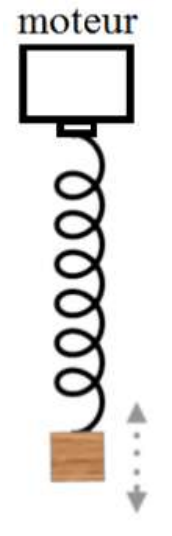
\includegraphics[width=0.45 \linewidth]{Figures/masse_ressort_general.png}
\end{minipage}

\vspace{0.3cm}

\noindent\textbf{Justification :} \hrulefill \\[2.5ex]
\rule{\linewidth}{0.4pt} \\[2.5ex]
\rule{\linewidth}{0.4pt}
\vfill